As explained in the background section, it is nearly impossible to differentiate the rendering process of a system not built for that purpose, but is a requirement when performing parameter estimation using gradient descent. To solve this, we propose building a back-end renderer in a framework that is automatically differentiable in addition to the normal forward rendering system. If this system is carefully setup to mimic the main forward rendering process, finding optimal parameters to the back-end rendering function will simultaneously solve the problem of finding parameters to the forward rendering function. In the overview of our system shown in Figure \ref{fig:SystemOverview}, these two parts are displayed; the forward rendering framework and a differentiable version used in parameter estimation. The user-facing forward rendering is performed with OpenGL, a popular API for rendering 2D and 3D graphics while the back-end renderer is implemented in Python using PyTorch. To estimate parameters of the functions constituting a procedural texture, the iterative optimization algorithm \textit{Stochastic Gradient Descent} is used. As explained in section \ref{sec:StochasticGradientDescent} on SGD, this algorithm relies on being able to find gradients of a loss function which, in our case, would measure the visual difference between a user's input target image and the image rendered from our back-end renderer. To assist users in designing procedural texture models, we have implemented a graphical node editor, where each node keeps a reference to both an OpenGL shader, and an equivalent shader implemented in PyTorch. The resulting node graph is a tree-like data structure that visualizes data flowing from node outputs into node inputs of connected nodes. In this chapter, each part of the system will be explained and motivated in detail, ending with a presentation of our graphical user interface used to control \dipter{}.

\begin{figure}[h]
    \centering
    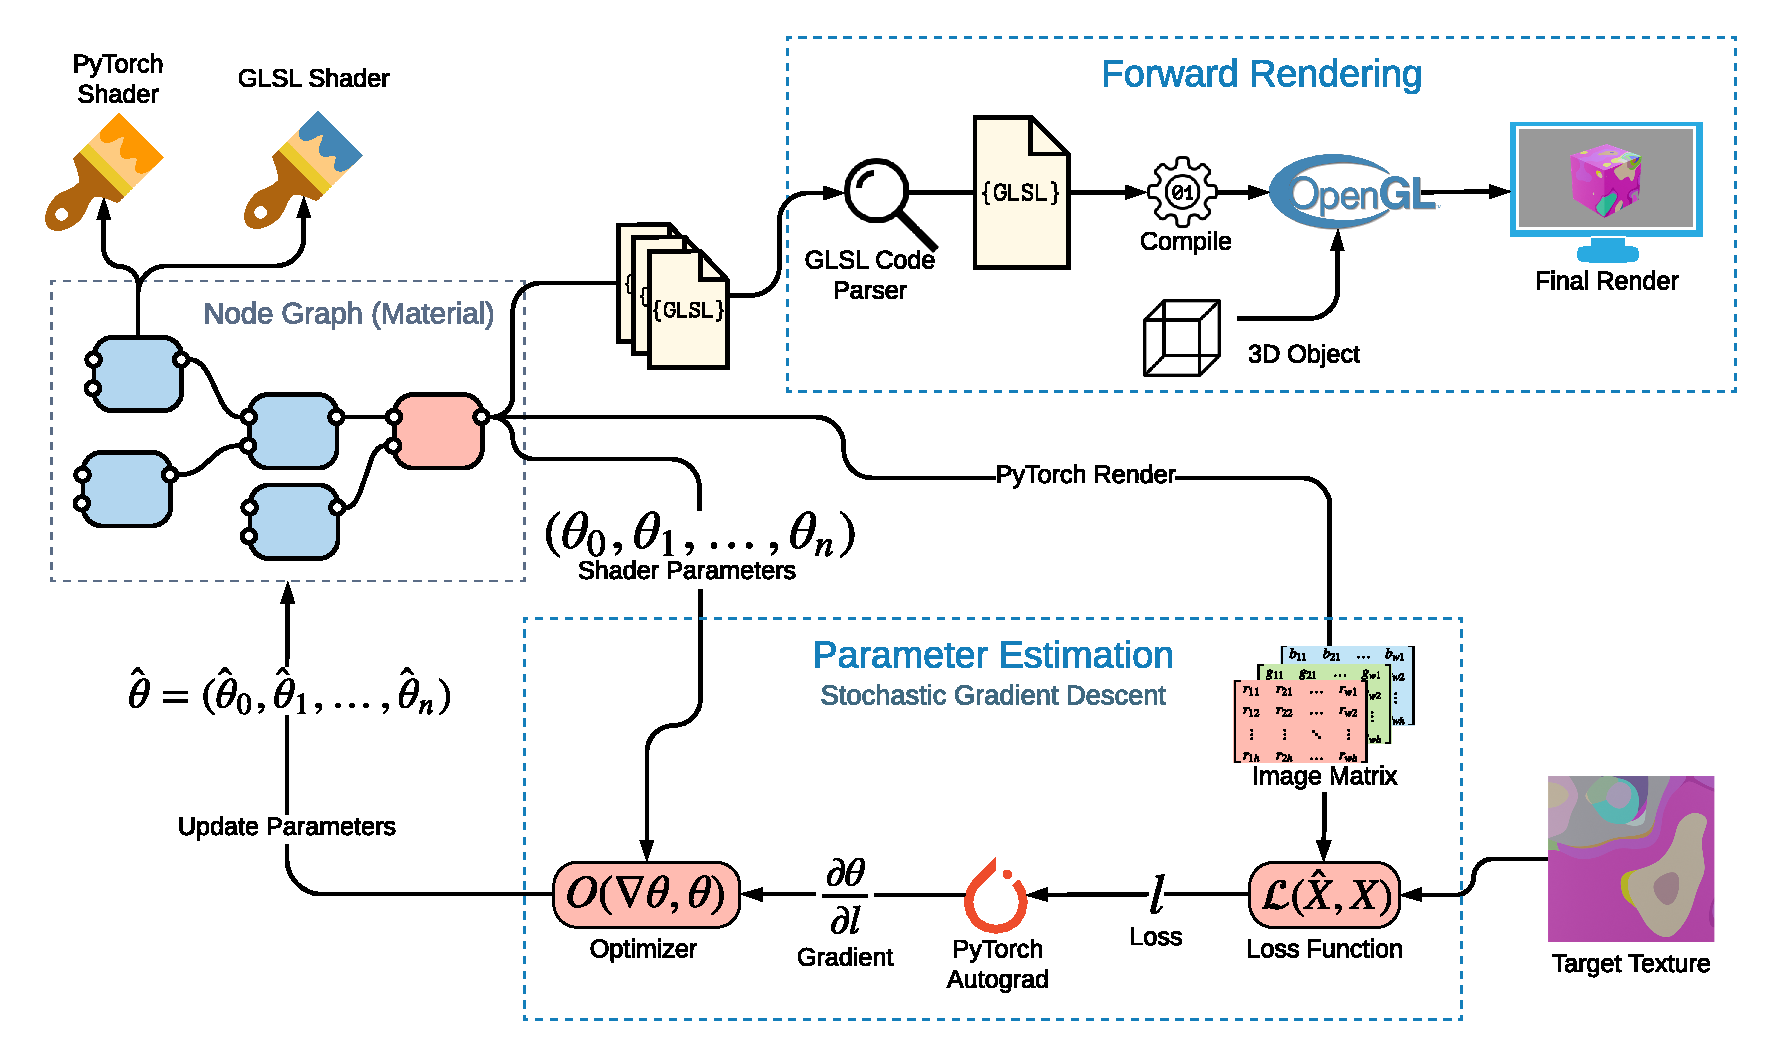
\includegraphics[width=1.0\textwidth]{img/method/System Overview.pdf}
    \caption{Overview of our forward and inverse rendering framework. A user starts by designing a composite shader using the node editor interface. Each node keeps a reference to two versions of the same shader, one for rendering and one for parameter estimation. The GLSL code of each node is parsed, assembled and compiled and sent to OpenGL for rendering. The optional parameter estimation is run in a loop where each iteration, a new rendered image and rendering parameters are used to estimate a better set of parameters, striving to reduce the loss.}
    \label{fig:SystemOverview}
\end{figure}

\section{Node Graph}

Function composition in procedural texturing systems is often illustrated as a node graph, where nodes represent a procedural function. More specifically, this graph is a \textit{directed acyclic graph}, where data flows from the leaf nodes up to the root, the \textit{Material Output Node}, so called because the resulting procedural texture is also referred to as a \textit{material}. The graph is \textit{directed} because data can only flow in one direction, from an output socket into an input socket, and \textit{acyclic} because any nodes connected in a loop would give rise to infinite recursion. An example of such a node graph is illustrated in Figure \ref{fig:NodeGraph}. The root node, a Material Output Node, is a specialized node in \dipter{} for a specific shader called the \textit{material output shader}. This shader acts as the \texttt{main} function in many programming languages, the entry point of execution, as explained in section \ref{sec:ImplementationProceduralShadingGLSL}, and rendering in Python must be initialized from this node. The function accepts one input that the user can not manually set, a generated pixel color which must be fed from another node.

\begin{figure}[h]
    \centering
    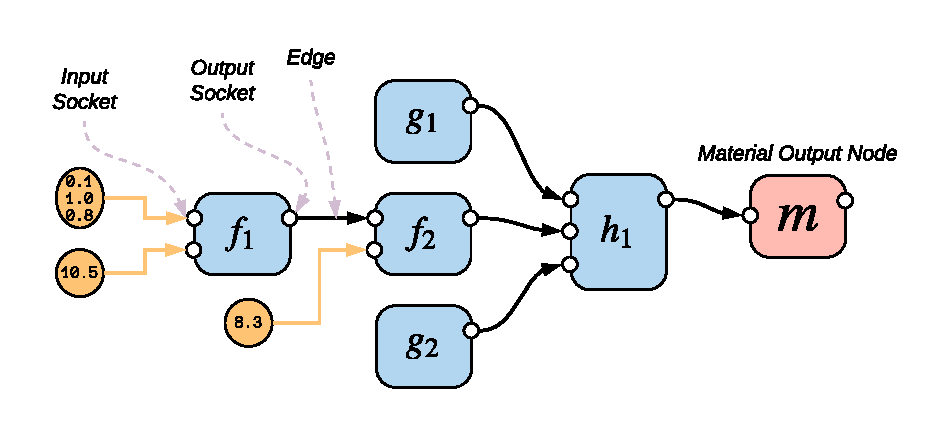
\includegraphics[width=0.9\textwidth]{img/method/Node Graph.pdf}
    \caption{An example procedural texture model represented as a node graph where yellow nodes represent user controlled input. The material output node is the root of the graph, marked in red.}
    \label{fig:NodeGraph}
\end{figure}

The number and type of input sockets of a node are entirely dictated by the shader function it represents and if not connected to another node, its value can be set by the user. The only exception being the coordinates of the rendered object which is handled internally and is not user controllable. In Figure \ref{fig:NodeGraph} the different functions the nodes represent are printed inside them, where some nodes represent the same function like $f_1$ and $f_2$. The resulting composite procedural texture function $m$ is shown in Equation \ref{eq:NodeGraphCompositeFunction}, omitting the fragment position arguments.

\begin{equation}
    m = h_1(g_1(), f_2(f_1(\left[0.1, 1.0, 0.8\right], 10.5), 8.3), g_2())
    \label{eq:NodeGraphCompositeFunction}
\end{equation}



\section{Forward Rendering}\label{sec:RenderingInOpenGL}

To render procedural textures onto objects we chose OpenGL, a popular and mature graphics API that is fairly easy to set up and integrate into our project. OpenGL comes with all the tools for rendering textures, procedural or not, onto both 2D and 3D objects and is highly optimized for this task. A reasonable question to ask at this point however, is why we even need a separate forward rendering setup at all if our differentiable renderer is designed to render the same result, and the reason is twofold; speed and portability. First of all, our back-end implementation is nowhere near as fast as OpenGL. Even if PyTorch has support for GPU acceleration, the overhead of differentiability and the fact that it is not specifically optimized for graphical calculations makes it too slow for real time rendering of anything but the simplest procedural textures, but performs well enough for parameter estimation. In the near future however, this might change as the team behind PyTorch is developing their own differentiable 3D renderer \cite{facebookresearch_2020_facebookresearchpytorch3d}. Lastly, the procedural textures built in our system can be exported and used in any other system that supports shaders written in GLSL. The Python code in our back end is unique to our system, and can not easily be incorporated elsewhere.

\subsection{OpenGL Shader}\label{sec:MethodOpenGLShader}

Procedural textures are rendered in OpenGL using small programs called \textit{shaders}, written in the purpose-built language \textit{OpenGL Shading Language} or GLSL. Details on OpenGL's rendering pipeline, where different types of shaders are explained, can be found in section \ref{sec:OpenGLRenderingPipeline}. \dipter{} mainly deals with fragment shaders which are applied to each fragment or pixel on an object, coloring them according to a function implemented in GLSL. The normalized coordinate of the point on the surface of the 3D object that is covered by the 2D fragment is an important input parameter to the fragment shader. It is calculated by the vertex shader, then interpolated and passed down for each fragment as explained in section \ref{sec:Interpolation}. In our system, this is the sole purpose of vertex shaders, and thus the same vertex shader is used for all types of procedural texture models and only has to be compiled once. Therefore, when we refer to a ''shader'' we refer to the fragment shader. Conceptually, a shader is nothing more than a function applied to each point $p$ on an objects surface that takes a set of optional parameters $\Vec{\theta}$ and the normalized coordinates of $p$ as input, and outputs a color for $p$ calculated from the input parameters, as shown in Figure \ref{fig:OpenGLShader}.


\begin{figure}
    \centering
    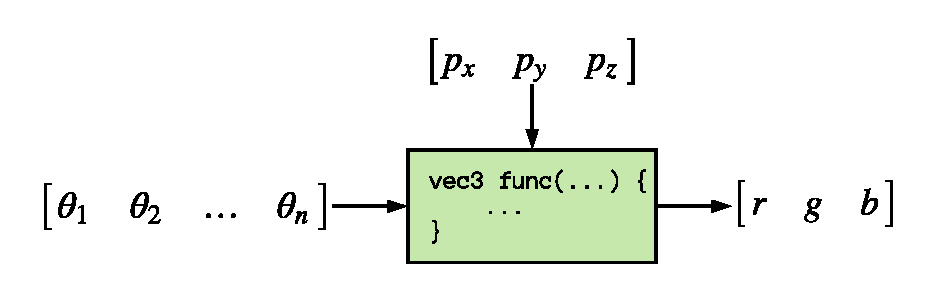
\includegraphics[width=0.9\textwidth]{img/method/Shader Diagram.pdf}
    \caption{A shader in \dipter{}'s forward rendering system is a function, applied to every point $p$ on an objects surface, that takes the normalized coordinates of $p$ and optional parameters $\Vec{\theta}$ as input, and outputs a color vector for $p$.}
    \label{fig:OpenGLShader}
\end{figure}


\subsection{Composing Shaders}\label{sec:MethodComposingShaders}

Much of the power of procedural textures comes from the fact that they are just functions, and as such can be composed and reused as explained in section \ref{sec:BackgroundProceduralTextures}. Unfortunately however, neither OpenGL nor GLSL have any support for shader composition or even code reuse. The latter can fairly easily be supported by implementing a custom preprocessor directive that simply prepends needed source code to a GLSL shader source file before compilation, see section \ref{sec:ImportPreprocessorDirective} on its implementation. Supporting dynamic function composition from Python at run-time however is more complex as GLSL is a compiled language, forcing us to recompile the shader source code each time a change to the node graph's structure is introduced. Furthermore, due to OpenGL restricting us to a single source file for our fragment shader, code from different files need to be assembled into a single file at run-time before compilation. To achieve this, we have built a custom parsing engine that reads and parses GLSL source files once, breaking down files, functions and arguments into Python objects. This code is dynamically reassembled and recompiled according to the structure of the node graph that a user has designed. OpenGL shaders accept input during runtime using so called \textit{uniforms} which have to be uniquely named. This can be tricky when a large node graph is interpreted, as each unconnected node input will be turned into a uniform in the resulting single file source code. If all nodes are of different types this does not pose much of a problem, but as nodes of the same type use the same code (and thus the same underlying argument names), an additional system to ensure unique uniform names is required. Therefore, each node of the same type is assigned a number that is unique within that type, which the uniform name is based on, see section \ref{sec:ImplementationProceduralShadingGLSL} for details.


\section{Differentiable Rendering}\label{sec:RenderingInDiPTeR}

While designing shaders in OpenGL is fairly easy using GLSL, reusing code and composing shaders dynamically poses a real challenge. For our differentiable shading the problem is essentially reversed, as setting up a rendering system that can reliably mimic the OpenGL renderer is difficult, while composing shaders is trivial and requires no parsing, as dynamically composing functions is innately supported by the Python programming language.

While OpenGL is a fully fledged computer graphics framework, our Python rendering engine is implemented as a simplified and highly specialized differentiable 2D procedural texture rendering engine. No 3D support is needed, as it is only used for parameter estimation by way of 2D texture similarity optimization. Furthermore, it assumes uniform directional lighting, meaning lighting is essentially not calculated, as we want to focus on reproducing underlying texture patterns and colors and parameters governing lighting is not necessarily part of the procedural texture function. By default, OpenGL includes a fourth color channel for opacity which we ignore as it is too ambiguous to be used in inverse rendering and thus we handle all images as having three channels.

To be able to differentiate the rendering procedure reliably and dynamically, we need to utilize automatic differentiation. Therefore, we implemented our differentiable renderer using Facebook's machine learning framework \textit{PyTorch} that features a built in automatic differentiation engine \cite{paszke_2019_pytorch}. A few other candidates were considered early on, like Google's automatic differentiator \textit{Jax} \cite{bradbury_2018_jax}. This framework has the advantage that it can automatically differentiate code that is almost identical to normal Python or Numpy syntax, whereas most other frameworks require the user to implement code with a specific syntax, a sort of mini-language. Additionally, TensorFlow was temporarily evaluated, but both frameworks were found to be slightly slower and not as robust as PyTorch.

As explained, an important requirement when designing PyTorch shaders is that for a specific parameter set and procedural texture model, both OpenGL and our PyTorch renderer should produce the same 2D texture matrix. Therefore, the simplest way to perform shading would be to iteratively call a shader function, or composition of shader functions, on each pixel of the 2D plane being rendered, mimicking the OpenGL shader in section \ref{sec:MethodOpenGLShader}. This approach in PyTorch is explained in section \ref{sec:MethodIterativeRendering}, but proves very inefficient, why a second much more efficient but unfortunately less readable solution was devised, dubbed \textit{matrix shading}. However, seeing as the rendering times were cut by upward a thousand times, some decrease in readability was deemed a justifiable sacrifice. 


\subsection{PyTorch Shader}

Each OpenGL shader has an associated Python class in \dipter{} which keeps a reference to the GLSL source file. This class will parse the GLSL source code, compile it as well as run tests to ensure compatibility between the two implementations. Additionally, a Python shader class needs to communicate to our system what inputs the shader function accepts and their datatype (used by the node graph subsystem) as well as the actual PyTorch implementation of the GLSL shader function. How the shade function is translated from GLSL into PyTorch's own mini-language is explained in section \ref{sec:ImplementationPyTorchShader}. As in other languages, GLSL comes with a standard library of useful functions that are automatically available when writing shaders and has to be reimplemented in Python. Fortunately, the details behind the mathematical implementation of many of these functions are revealed in the GLSL documentation, but not always. It is therefore important to run tests on each implemented library function to assure that it returns the same result as the GLSL version.

\subsubsection{Generating Fragment Coordinates}

By default convention, the pixel positions in OpenGL are located at \textit{half-pixel coordinates}, meaning that the actual coordinate for a pixel is the position of the center of that pixel \cite{segal_2013_the}. In Python, this means that the index of an element in the rendered image matrix does not directly correlate with the fragment coordinate. This does not matter much if the resolution is high, as the maximum error of the fragment position we can get if we incorrectly assume that the coordinates are given by the lower left corner of a pixel is half a pixel, a fraction $\frac{1}{2r}$ of the image, where $r$ is the pixel resolution in some direction. Let $w$ and $h$ be the image width and height in pixels and $(x,y)$ the index of a pixel element in the matrix, where $0 \leq x \leq w-1$ and $0\leq y \leq h-1$. In general, a pixel's (or fragment's) position at index $(x,y)$ is given by equation \ref{eq:UnnormalizedFragPos}. Note that this is the coordinate in three dimensions.

\begin{equation}\label{eq:UnnormalizedFragPos}
p(x,y) = \begin{bmatrix}x + \frac{1}{2w}, & y + \frac{1}{2h}, & 0\end{bmatrix}
\end{equation}

In our system however, we are only interested in the normalized fragment coordinate, so as to be independent of the rendering resolution. The normalized fragment coordinate \texttt{frag\_pos} is given by equation \ref{eq:FragPos}. Because we need to model our shaders in Python as similar as possible to the OpenGL standard, this is used when generating fragment positions.

\begin{equation}\label{eq:FragPos}
    \fragpos(x,y) = \begin{bmatrix}\frac{x}{w} + \frac{1}{2w}, & \frac{y}{h} + \frac{1}{2h}, & 0\end{bmatrix}
\end{equation}


\subsubsection{Iterative Shading}\label{sec:MethodIterativeRendering}

Iterative shading attempts to model the way shaders operate in OpenGL, where a fragment shader is called for each fragment (effectively pixel) independently and returns a color for that one fragment. To render an image, we first need to define its width and height in pixels and create an empty matrix of shape $(width, height, 3)$ as our image placeholder. Then, each position in the matrix is assigned to the output of the render function, where the normalized pixel coordinate \texttt{frag\_pos} is relative to the position in the matrix while the other arguments are kept constant. This algorithm is explained in pseudocode in Algorithm \ref{alg:IterativeRendering}. 

While this implementation is straight forward and easily translated from GLSL, the two nested Python for loops become a major performance bottleneck. All PyTorch functions are implemented and highly optimized in a C++ back end while Python for loops are notoriously slow. Furthermore, some shaders do not use the \texttt{frag\_pos} variable, and will thus have the same output for each pixel. Calling the shader function $width \times height$ times, when we could call it once and replicate the output over the entire image, is a huge waste of time. Another, even worse implication is the fact that PyTorch will add a node to the computational graph for each call to a PyTorch function. As such, this approach will add $width \times height$ duplicate operation nodes to the graph, making it much slower to traverse in the backward step as well as memory inefficient. Using only built in PyTorch functions as far as possible can give a thousandfold performance boost, especially when rendering higher resolution images. How this is achieved is explained in the next section.

\begin{algorithm}
	\SetKwData{Img}{img}\SetKwData{Width}{width}\SetKwData{Height}{height}\SetKwData{Xs}{xs}\SetKwData{Ys}{ys}\SetKwData{X}{x}\SetKwData{Y}{y}\SetKwData{FragPos}{frag\_pos}\SetKwData{Params}{params}
	\SetKwFunction{Shade}{Shade}\SetKwFunction{GenerateFragPos}{GenerateFragPos}
	\SetKwInOut{Input}{Input}\SetKwInOut{Output}{Output}
	
	\Input{A shade function \Shade, a set of parameters \Params and an image size tuple (\Width, \Height).}
	\Output{A matrix of size $\Width \times \Height \times 3$ containing the pixel data for the rendered image.}
	
	\BlankLine
	Initialize \Img as empty matrix of size (\Width, \Height, 3)\;
	
	\For {\X $=0$ \KwTo \Width}{
		\For{\Y $=0$ \KwTo \Height}{
			\FragPos $\leftarrow$ \GenerateFragPos{x,y}\;
			\Img[\X, \Y] $\leftarrow$ \Shade{\FragPos, \Params} \;
		}
	}
	\Return \Img\;
	\caption{Iterative rendering algorithm}
	\label{alg:IterativeRendering}
\end{algorithm}

\subsubsection{Matrix Shading}\label{sec:MethodMatrixImplementation}

One major disadvantage to PyTorch is that it does not have a \texttt{map}-function that can apply a function to each position in a matrix. This would solve our problem, as we could keep our iterative method while removing the need for slow Python loops. Instead, we can generate input and output parameters for every pixel simultaneously in a matrix the same size as the final rendered image. PyTorch uses its own data structure called a \texttt{Tensor} that represents data of any shape or dimension of any primitive Python type. The functions in the PyTorch library operate on these tensors element-wise, which we can utilize to calculate parameters and color data for the entire image in one call to the shade function. Any parameter of size $d$, be it a scalar where $d=1$ or a color vector where $d=3$, can be extended to a tensor of size $(width, height, d)$ to represent that parameter over the entire image. The fragment coordinates can now be generated once in the superclass and used by all shaders as a tensor of size $(width, height, d=3)$, where each element is a vector $[p_x,  p_y,  p_z]$. The output of a shader function is now not only the color of a single pixel but the color of all pixels, in other terms; the fully rendered image. Thanks to PyTorch's element-wise operators, the implementation does not have to change at all in some cases, and in most cases, it is only a matter of handling the extra dimensions. The performance gains are particularly significant for shaders that do not utilize the fragment coordinates, and therefore have a uniform color output across the image. In these shaders the color only have to be calculated once and then repeated using PyTorch's \texttt{repeat} function instead of running the shader thousands of times, once for each pixel, like in the iterative method. The other advantage of this method is that the resulting computational graph is much smaller, as each operation only has to be added once.


For visual reference, the fragment coordinates matrix is shown in equation \ref{eq:FragPosMatrix}. Let $f(x,y)$ denote the function that generates the fragment coordinate in equation \ref{eq:FragPos}, at each image integer index $(x,y)$, and let $f_x$, $f_y$, $f_z$ denote functions that return the $x$,$y$, and $z$ coordinates returned by $f$, respectively. The equation shows the matrix $F$ that contains all the fragment positions, such that each position $i,j$ in the matrix contains the vector $f(i,j)$. 
The matrix rendering method has an important speed advantage, but there does exist a truly limiting drawback when it comes to loops, where the loop count is dictated by an argument to the shader function. As mentioned, all arguments are matrices, and can therefore not be used as arguments to most Python control flow such as \texttt{if}-statements and \texttt{for}-loops, but some of these cases can be solved by using PyTorch alternative functions, see section \ref{sec:ImplementationPyTorchShader}.

\begin{equation}\label{eq:FragPosMatrix}
	\begin{aligned}
		F[:,:,0] &= 
		\begin{bmatrix} 
			f_x(0,0)    & f_x(1,0)  & \dots     & f_x(w,0)  \\
			f_x(0,1)    & f_x(1,1)  & \dots     & f_x(w,1)  \\
			\vdots      & \vdots    & \ddots    & \vdots    \\
			f_x(0,h)    & f_x(1,h)  & \dots     & f_x(w,h)  
		\end{bmatrix} \\
		F[:,:,1] &= 
		\begin{bmatrix} 
			f_y(0,0)    & f_y(1,0)  & \dots     & f_y(w,0)  \\
			f_y(0,1)    & f_y(1,1)  & \dots     & f_y(w,1)  \\
			\vdots      & \vdots    & \ddots    & \vdots    \\
			f_y(0,h)    & f_y(1,h)  & \dots     & f_y(w,h)  
		\end{bmatrix} \\
		F[:,:,2] &= 
		\begin{bmatrix} 
			0    & 0  & \dots     & 0  \\
			0    & 0  & \dots     & 0  \\
			\vdots      & \vdots    & \ddots    & \vdots    \\
			0    & 0  & \dots     & 0  
		\end{bmatrix}
	\end{aligned}
\end{equation}

% \begin{algorithm}[H]
% \SetKwData{D}{D}\SetKwData{Width}{width}\SetKwData{Height}{height}\SetKwData{T}{t}\SetKwData{V}{V}\SetKwData{FP}{frag\_pos}
% \SetKwFunction{Func}{Func}
% \SetKwInOut{Input}{Input}\SetKwInOut{Output}{Output}

% \Input{A iteration count parameter D.}
% \Output{A rendered image matrix of size $\Width \times \Height \times 3$.}

% \BlankLine
% Initialize V to matrix of zero vectors.\;
% Initialize \FP to fragment coordinates matrix.\;

% \For {\T $=0$ \KwTo \D}{
%     \V = \V + \Func{\FP}\;
    
% }
% \Return \V\;
% \caption{An example of a shader that is very difficult to translate to our matrix form, as \texttt{D} is a matrix with a potentially different value for each pixel, while in an iterative method, the shade function would be executed for each pixel, and \codeinline{D} would simply be an integer scalar tensor.}
% \label{alg:MatrixMethodForProblem}
% \end{algorithm}

\subsection{Composing Shaders}

As Python is our main programming language and the shaders are defined in Python, shaders are already symbolically composed via the node graph. Rendering a composed shader can therefore be easily achieved by traversing the node graph in a correct order and using the output of shaders as input to other connected shaders. Rendering with composite shaders have to be initialized from a node in the graph rather than a shader, as shaders are isolated units, in essence a single function, without any references to other shaders.

The node graph is traversed in depth first order starting from the Material Output root node. Rendering is recursive, and for current node $N$, the algorithm starts by checking each input socket if it is connected and if so, the connected node is recursively rendered and the output is saved to be used as a parameter for $N$s shading function. If the socket is not connected, the parameter value is fetched from the input widget, set by the user in the graphical interface. The unconnected parameters are saved in a dictionary and constitutes the procedural texture parameters $\vec{\theta}$ we want to optimize during parameter estimation. Finally, the shade function is called using the collected parameters and the rendered matrix is returned together with the parameter dictionary for $N$. For every recursive render call, this dictionary is extended until all connected nodes have been rendered and the parameter dictionary is complete for the graph. This algorithm is shown in Algorithm \ref{alg:PythonCompositeRendering}. The \texttt{Shade} function being called at the end is the shade function of the shader that the current node being rendered contains. The call to \texttt{GetUniqueUniform} is needed when translating the parameter values to OpenGL in order to know which parameter value belongs to which uniform.



\section{Parameter Estimation}

Parameter Estimation, also referred to as \textit{Texture Matching} in \dipter{}, is our subsystem that lets users automatically estimate parameters of a procedural texture model they designed in order to minimize the difference between a target bitmap texture and the procedural texture output. This is posed as an optimization problem, where the goal is to find optimal parameters $\Vec{\theta}^*$ such that they minimize a loss function $\loss(\Vec{\theta}^*)$. In our system however, we split the rendering of our procedural texture $\hat{X} = R(\vec{\theta})$ and the loss measurement $l=\loss(\hat{X},X)$ because in PyTorch, all operations performed on Tensors are tracked locally in the Tensor datastructure. This enables us to have the loss function only indirectly depend on the procedural parameters and instead be a function of two parameters, a Python rendered image and a user supplied target image. In other words, we can render the image in one function and calculate the loss in another function, but all operations performed on the parameters in either function will be registered in the Tensors. This is crucial, as it enables us to find the derivative $\frac{\partial \theta_i}{\partial l}$ of any parameter $\theta_i \in \vec{\theta}$ with respect to the final loss $l = \loss(\hat{X}, X)$, even though the loss function does not directly depend on parameter $\theta_i$. Parameter estimation is controlled through our texture matching GUI, see section \ref{sec:TextureMatcherInterface}.

\begin{algorithm}
	\SetKwProg{Fn}{Function}{}{end}\SetKwFunction{Render}{Render}%
	\SetKwData{Width}{width}\SetKwData{Height}{height}\SetKwData{Arg}{arg}\SetKwData{ParamsDict}{params\_dict}\SetKwData{Arguments}{arguments}\SetKwData{Socket}{socket}\SetKwData{Node}{node}\SetKwData{Value}{value}\SetKwData{PD}{pd}\SetKwData{Uniform}{uniform}\SetKwData{Root}{root\_node}
	\SetKwFunction{GetInputSockets}{GetInputSockets}\SetKwFunction{GetConnectedNode}{GetConnectedNode}\SetKwFunction{GetArg}{GetArg}\SetKwFunction{GetValueFromSocket}{GetValueFromSocket}\SetKwFunction{GetUniqueUniform}{GetUniqueUniform}\SetKwFunction{Shade}{Shade}
	
	
	\Fn{\Render{\Width, \Height}}{
		Initialize \ParamsDict as empty dictionary\;
		Initialize \Arguments as empty dictionary\;
		
		\For{\Socket $\in$ \GetInputSockets{}}{
			\Arg $\leftarrow$ \GetArg{\Socket}\;
			\Uniform $\leftarrow$ \GetUniqueUniform{\Arg} \;
			\eIf{\Socket is connected}{
				\Node $\leftarrow$ \GetConnectedNode{\Socket}\;
				\tcp{recursive rendering}       
				\Value, \PD $\leftarrow$ \Node.\Render{\Width, \Height}\;
				Update \ParamsDict with \PD\;
			}{
				\Value $\leftarrow$ \GetValueFromSocket{\Socket}\;
				Add \Value to \Arguments with key \Arg\;
			}
			Add \Value to \ParamsDict with key \Uniform \;
		}
		
		\Return \Shade{\Arguments}, \ParamsDict \;
	}
	\caption{Recursive rendering algorithm for composite Python shaders.}
	\label{alg:PythonCompositeRendering}
\end{algorithm}


\subsection{Loss Functions}\label{sec:MethodLossFunctions}

% \textbf{X and $\hat{X}$ are both clamped before being compared because otherwise they wont correspond to what is being rendered! Both openGL and matplotlib/pyqtgraph clamp values to 0,1.}
We make three loss functions available to users: a simple Mean Squared Error loss, Squared Bin Loss as well as a more sophisticated Neural Loss. The MSE loss function works exactly as described in section \ref{sec:LossFunctions} and is very fast and exact, as it measures similarity between individual pixels. It can perform well for very simple procedural textures where an exactly matching result is possible to obtain. In the general case however, this will not be the case, especially not when noise is used in the textures. The Squared Bin loss function is similar to an MSE loss function, but divides the image into regions or bins of $N\times N$ pixels and calculates the average color of each bin, before finally returning the mean squared error of the averages. This loss function can work well for finding general patterns in an image, but can fail within the regions. Making the regions larger makes it less sensitive to noise, but performs worse within regions, and if the regions are made too small, the loss function will exhibit the same traits as the normal MSE. 

Building on findings by Guo et. al., an even better solution should be to utilize machine learning to automatically unveil the underlying patterns in the textures, and directly comparing them \cite{guo_2019_a}. This type of loss function is dubbed a Neural Loss, as the general idea is to pass the images through a neural network, where image features will be extracted by the different layers in the networks, as explained in section \ref{sec:LossFunctions}. This loss function is much more spatially independent than the other two and should focus more on the general look of the textures. For example, the other two loss functions would be fairly bad at recognizing that two different textures of the same type of wood are similar, because locally, these textures can have very different color values. A neural loss function however, could extract features pertaining to the direction of the grain or the presence of knots. A comparison of the performances of these loss functions is found in section \ref{sec:EvalParameterEstimationSpeed}.

\subsection{Gradient Descent}


Gradient Descent is performed much like described in Algorithm \ref{alg:GradientDescent}. Each iteration, an image is rendered using parameters $\vec{\theta}$ and a loss value is calculated between the rendered image $\hat{X}$ and the target image $X$. All operations performed directly on the parameters in $\vec{\theta}$ or on variables created as a result of an operation on a parameter in $\vec{\theta}$ are registered in the computational graph. The next step is to utilize PyTorch's automatic differentiation package to traverse the computational graph backwards from the loss, calculating gradients for each of our parameters. Given the gradients, the direction of the steepest ascent of the loss function relative to each parameter's dimension is known. A small gradient $g_i$ for parameter $\theta_i$ means that only a small correction of this parameter is needed in order to reach an optimal loss value, and vice versa. Lastly, it is up to the chosen optimizer to calculate new values for each parameter based on its gradient. Before the next iteration is started, the rendered Python image is updated in the graphical interface and likewise the new parameters are sent to the OpenGL shader program, rendering the updated texture. This is an important visual tool and enables users to verify that the algorithm is correctly optimizing the parameters. Additionally, the new loss value is plotted to display the progress over time. The algorithm terminates when the maximum number of iterations has been reached, or the loss value is less than a specified threshold. The new parameter values can be applied to the procedural texture, if the results are satisfying. 

\section{Graphical User Interface}

While it is possible to build procedural textures and perform parameter estimation programmatically with our framework, it is faster and more convenient to interact with \dipter{} through our graphical user interface. The GUI is created using \textit{PyQt5}, the Python bindings for the popular C++ library \textit{Qt}, an extensive suite for cross-platform embedded and desktop UI development \cite{riverbankcomputing_2020_what,theqtcompany_qt}.

\subsection{Node Editor Interface}\label{sec:NodeEditorInterface}

Node graphs, and thereby procedural textures, are designed by the user in a \textit{node editor interface} shown in Figure \ref{fig:NodeEditorInterface}. This is a graphical user interface that lets users spawn nodes from a menu and drag edges to connect nodes' input and output sockets. Next to an unconnected input socket, a widget allows users to manually control parameter values of a node's shader. \dipter{} currently supports input values of a number of different types: integer or floating point numbers, colors by opening a color selector window and scalar vector input. To the right of the node editor is the OpenGL render area, where the procedural shader is rendered onto a chosen object in real time that can be rotated and zoomed by the user and any changes to input values or the structure of the graph will immediately be reflected in the rendering. A menu with available node types can be opened by right clicking the node editor area. Just above the node editor scene is a toolbar where users can create new materials by clicking the \emph{plus} button, as well as select a material to display from the drop-down list. \dipter{} also supports saving and loading materials to JSON format.
 
 
\begin{figure}[!h]
    \centering
    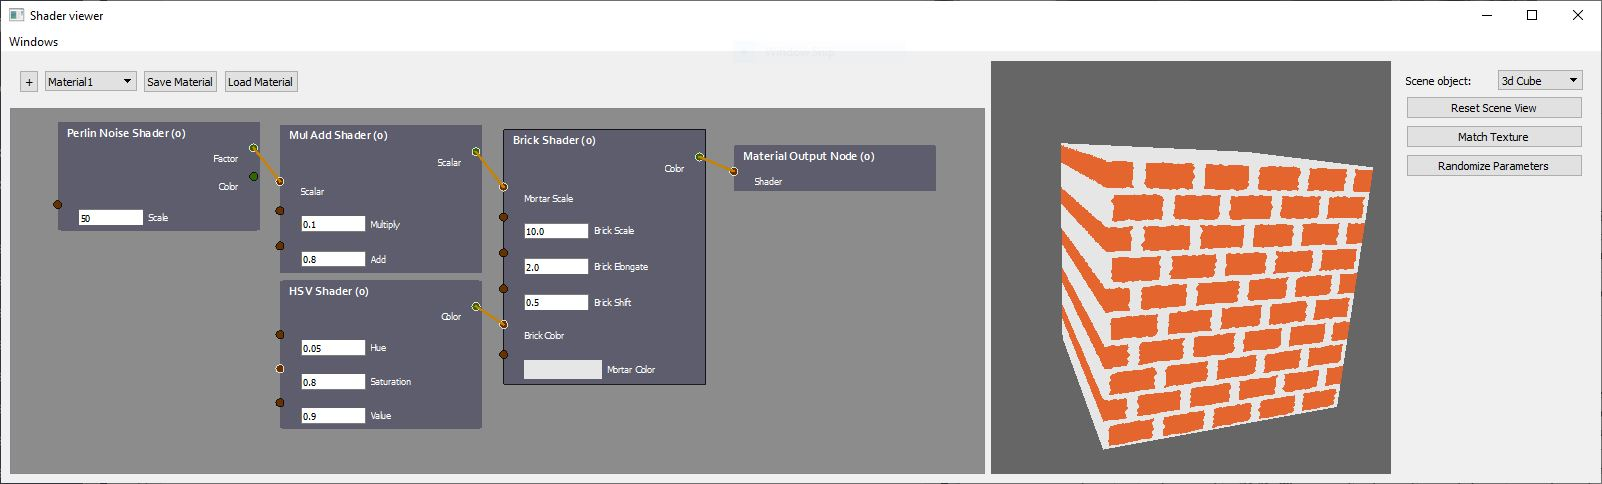
\includegraphics[width=.9\textwidth]{img/method/Node Editor.JPG}
    \caption{Node Editor Interface in \dipter{}. To the right of the node editor is the OpenGL rendering area, where the procedural texture is shown being rendered onto a cube.}
    \label{fig:NodeEditorInterface}
\end{figure}

\subsection{Texture Matcher}\label{sec:TextureMatcherInterface}

Parameter estimation is controlled by the user through our texture matching interface shown in Figure \ref{fig:TextureMatcherInterface}. Here, a user can control various aspects of the gradient descent algorithm such as maximum number of iterations or set a loss threshold that, once reached, signals the completion of the algorithm. Furthermore, the user can select the loss function and optimizer to be used in gradient descent and change their settings. These are the two components that have the largest influence on the success of the parameter estimation process. The loss function sets the upper bound of our result, as a loss of zero is the best outcome we can achieve and if that does not correspond to an optimal similarity between our two images, then the loss function is clearly not good enough. On the other hand, it is the optimizer's job to make sure this value is reached, or at least as close as possible. Apart from the settings panel, the interface is divided into four views. In the top left the procedural texture is shown as rendered by OpenGL, and in the middle, as rendered by the Python back end. Both of these views are updated each iteration and allows the user to assert that the two systems render a similar result and that the algorithm is progressing properly. The top right view displays the target image and hopefully, by the end of the last iteration, all three views will display visually similar images. Lastly, the bottom view plots the loss value versus iteration, hopefully showing a steady decline as the optimization progresses.


\begin{figure}[!h]
    \centering
    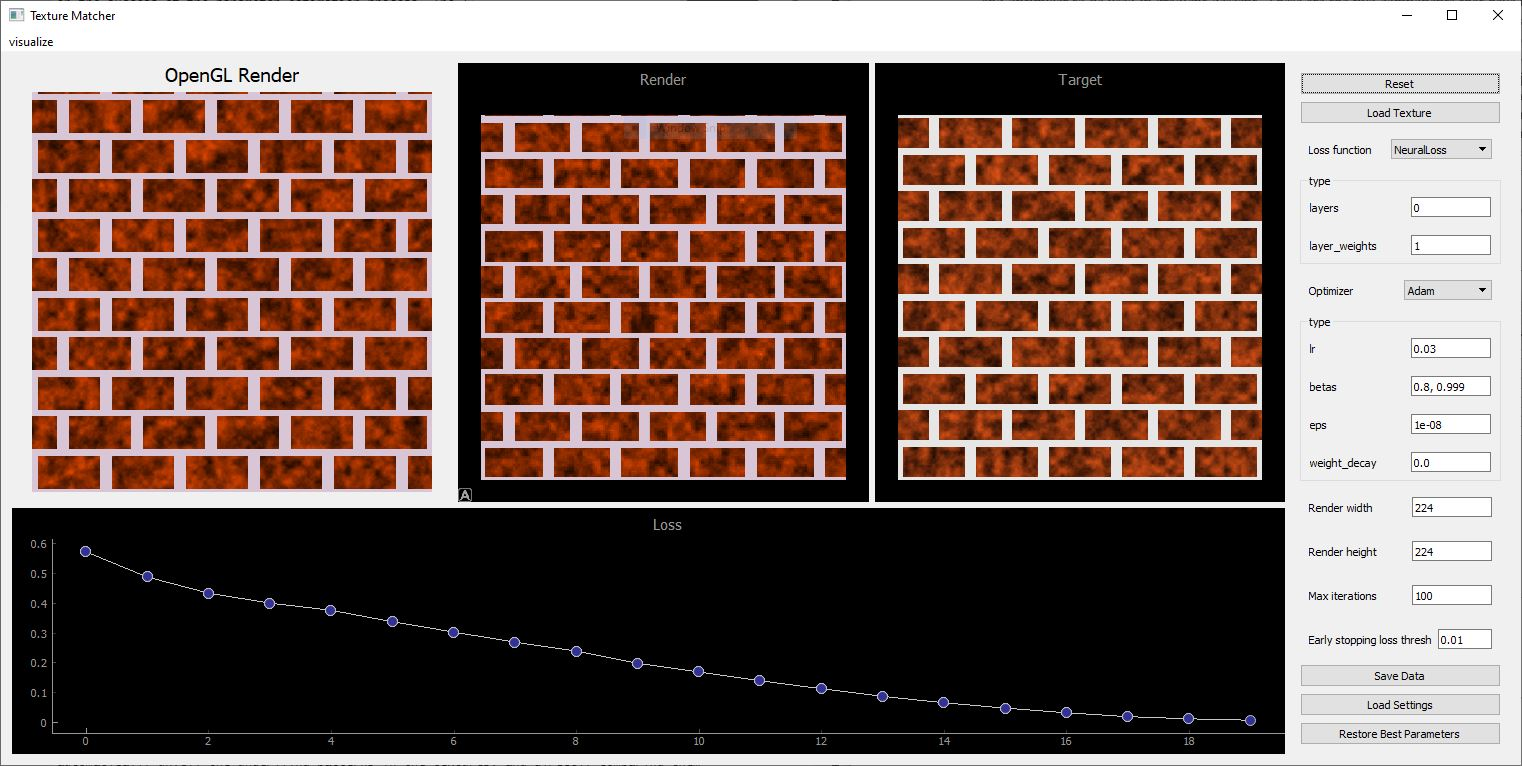
\includegraphics[width=.9\textwidth]{img/method/Texture Matcher.JPG}
    \caption{Graphical interface of the texture matcher, allowing the user to control parameter estimation. The loss has successfully converged to the threshold and all three views show a similar image.}
    \label{fig:TextureMatcherInterface}
\end{figure}

\subsection{Loss Visualizer}\label{sec:LossVisualizerInterface}

The loss value at the end of the gradient descent procedure will almost always be lower than the initial value. However, it is very possible that the final value is a local minima and that a better parameter estimation could be found. One way that this process can be debugged and analyzed is by explicitly plotting the loss for a range of parameter values as a surface plot. Unfortunately, it can only be visualized for two parameters at most, occupying the x- and y-axes, as the third axis is used by the loss value itself. Figure \ref{fig:LossVisualizer} shows the Loss Visualizer interface, where a user can select up to two parameters from their procedural texture in the list on the left and view the resulting, interactive loss surface. A user can also override the minimum and maximum values for each parameter, thereby restricting or expanding the parameter space. From this, it is possible to visually and manually find the optimal loss value relative to the selected parameters. Furthermore, the gradient descent progress can be plotted as a line on top of this surface, allowing the user to see exactly where the algorithm potentially got stuck. In Figure \ref{fig:LossVisualizer} we can clearly see that the gradient descent algorithm, marked with red dots, gets stuck in a local minimum ''valley'' and does not reach the minimum loss marked with a magenta \textit{plus} symbol.

\begin{figure}[!h]
    \centering
    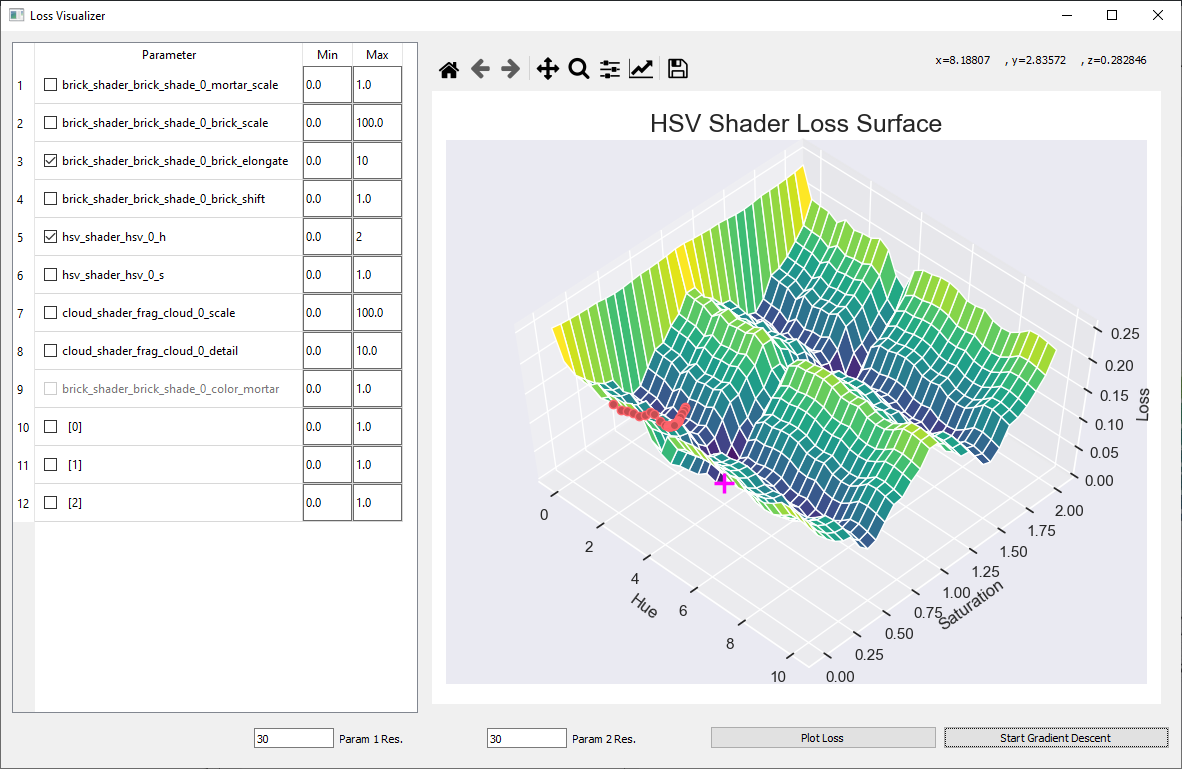
\includegraphics[width=.9\textwidth]{img/method/Loss Visualizer v3.PNG}
    \caption{Loss Visualizer interface showing available parameters and their value ranges to the left and the resulting loss surface to the right. The minimum loss value is marked with a magenta ''plus'' symbol.}
    \label{fig:LossVisualizer}
\end{figure}